\documentclass[a4paper,11pt,UTF8]{article}
\usepackage{ctex}
\usepackage{amsmath,amsthm,amssymb,amsfonts}
\usepackage{amsmath}
\usepackage[a4paper]{geometry}
\usepackage{graphicx}
\usepackage{microtype}
\usepackage{siunitx}
\usepackage{booktabs}
\usepackage[colorlinks=false, pdfborder={0 0 0}]{hyperref}
\usepackage{cleveref}
\usepackage{esint} 
\usepackage{graphicx}
\usepackage{ragged2e}
\usepackage{pifont}
\usepackage{extarrows}
\usepackage{mathptmx}
\usepackage{float}
\usepackage{caption}
\usepackage{bm}
\captionsetup[figure]{name={Figure}}
%opening
\title{科学计算引论作业(三)}
\author{谢悦晋 \quad U202210333}
\date{Sept 28th, 2023 }
\begin{document}
\maketitle
\noindent\textbf{3.3} 用改进的Cholesky分解法求解方程组
$$
\begin{pmatrix}5&-4&1&0\\-4&6&-4&1\\1&-4&6&-4\\0&1&-4&5\\\end{pmatrix}\begin{pmatrix}x_1\\x_2\\x_3\\x_4\end{pmatrix}=\begin{pmatrix}2\\-1\\-1\\2\end{pmatrix}
$$
解:\\
\textbf{Step 1}. 计算 $d_1,\boldsymbol{L}$ 的第 1 列元素
$$
\begin{aligned}d_1=a_{11},\quad l_{j1}=a_{j1}/d_1,\quad j=2,3,\cdots,4.\end{aligned}
$$
$$\Rightarrow
d_1=5,\begin{pmatrix}l_{11}\\l_{21}\\l_{31}\\l_{41}\end{pmatrix}=\begin{pmatrix}-1\\-1\\2\end{pmatrix}
$$
\textbf{Step 2}. 若 $\boldsymbol{D,L}$ 的前 $j-1$ 列元素已计算,则计算 $\boldsymbol{D,L}$ 的第 $j$ 列元素($\boldsymbol{D,L}$的结果在后面)
$$
\begin{aligned}
	&d_j=a_{jj}-\sum_{k=1}^{j-1}l_{jk}v_{jk},\quad v_{jk}=l_{jk}d_k,\\
	&l_{ij}=\left(a_{ij}-\sum_{k=1}^{j-1}l_{ik}v_{jk}\right)/d_j,\quad i=j+1,j+2,\cdots,4.
\end{aligned}
$$
\noindent\textbf{Step 3}. 求解下列系数矩阵为下三角形矩阵和上三角形矩阵的方程组
$$
LY=b,\quad DL^\mathrm{T}X=Y.
$$
获得原方程组的解 $X$.
\begin{figure}[H] 
	\centering 
	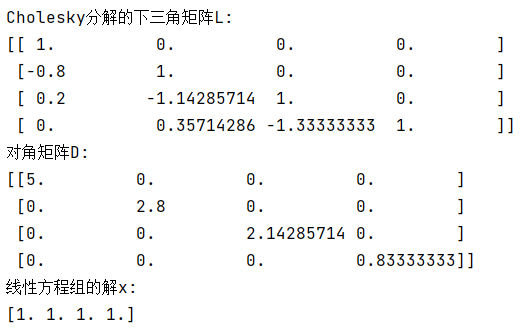
\includegraphics[scale=0.8]{kx3.3_1.png}
	\caption{代码运行图}
\end{figure}
\noindent 完整的Python代码如下:
\begin{figure}[H] 
	\centering 
	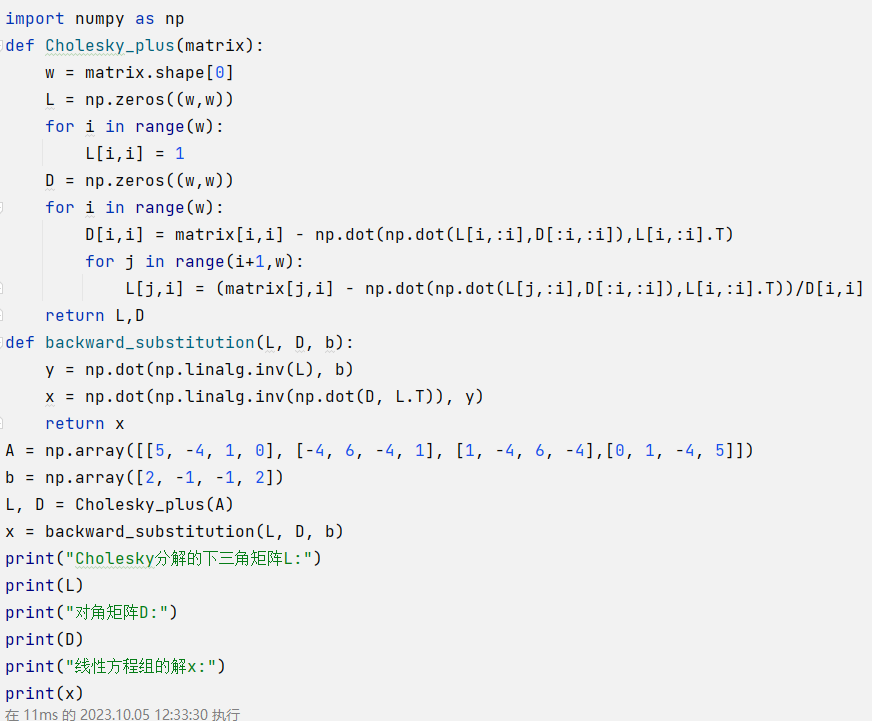
\includegraphics[scale=0.5]{kx3.3_2.png}
	\caption{Source Code}
\end{figure}
\textbf{3.4} 用追赶法求解三对角型方程组
$$
\begin{pmatrix}2&-1&0&0&0\\-1&2&-1&0&0\\0&-1&2&-1&0\\0&0&-1&2&-1\\0&0&0&-1&2\end{pmatrix}\begin{pmatrix}x_1\\x_2\\x_3\\x_4\\x_5\end{pmatrix}=\begin{pmatrix}1\\0\\0\\0\\0\end{pmatrix}
$$
求$Ax=f$等价于求$\begin{cases}Ly=f\\Ux=y\end{cases}$ 其中$f=\left(b_{1},f_{2},\ldots,f_{n}\right)^{T}$,故有:
$$
\begin{bmatrix}1&&&&\\p_2&1&&&\\&p_3&1&&\\&&\ddots&\ddots&\\&&&p_n&1\end{bmatrix}\begin{bmatrix}y_1\\y_2\\y_3\\\vdots\\y_n\end{bmatrix}=\begin{bmatrix}f_1\\f_2\\f_3\\\vdots\\f_n\end{bmatrix} \\
$$
解得$\begin{cases}y_1=f_1\\y_i=f_i-p_iy_{i-1}\quad\left(i=2,\ldots,n\right)\end{cases}\\$
再由
$$
\begin{bmatrix}q_1&c_1&&&\\&q_2&c_2&&\\&&\ddots&\ddots&\\&&&q_{n-1}&c_{n-1}\\&&&&q_n\end{bmatrix}\begin{bmatrix}x_1\\x_2\\\vdots\\x_{n-1}\\x_n\end{bmatrix}=\begin{bmatrix}y_1\\y_2\\\vdots\\y_{n-1}\\y_n\end{bmatrix}\\
$$
解得$\quad\left\{\begin{aligned}x_n&=\frac{y_n}{q_n}\\x_i&=\frac{y_i-c_ix_{i+1}}{q_i}\quad(i=n-1,\ldots,1)\end{aligned}\right.$\\
这是追赶法的主要过程,下面给出Python代码实现及运行结果:
\begin{figure}[H] 
	\centering 
	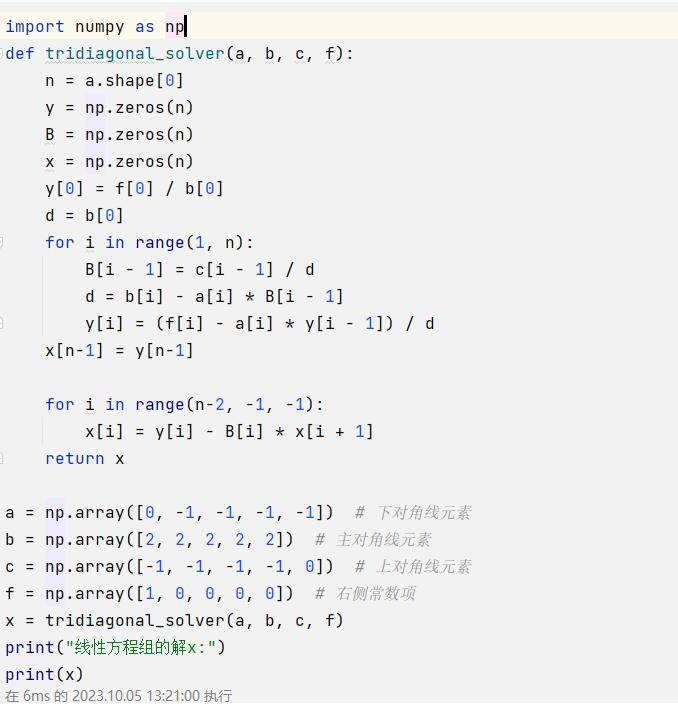
\includegraphics[scale=0.7]{kx3.4.jpg}
	\caption{Source Code}
\end{figure}
\begin{figure}[H] 
	\centering 
	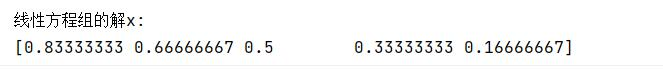
\includegraphics[scale=0.8]{kx3.4_1.jpg}
	\caption{Result}
\end{figure}
\end{document}